% Options for packages loaded elsewhere
% Options for packages loaded elsewhere
\PassOptionsToPackage{unicode}{hyperref}
\PassOptionsToPackage{hyphens}{url}
\PassOptionsToPackage{dvipsnames,svgnames,x11names}{xcolor}
%
\documentclass[
  letterpaper,
  DIV=11,
  numbers=noendperiod]{scrartcl}
\usepackage{xcolor}
\usepackage{amsmath,amssymb}
\setcounter{secnumdepth}{-\maxdimen} % remove section numbering
\usepackage{iftex}
\ifPDFTeX
  \usepackage[T1]{fontenc}
  \usepackage[utf8]{inputenc}
  \usepackage{textcomp} % provide euro and other symbols
\else % if luatex or xetex
  \usepackage{unicode-math} % this also loads fontspec
  \defaultfontfeatures{Scale=MatchLowercase}
  \defaultfontfeatures[\rmfamily]{Ligatures=TeX,Scale=1}
\fi
\usepackage{lmodern}
\ifPDFTeX\else
  % xetex/luatex font selection
\fi
% Use upquote if available, for straight quotes in verbatim environments
\IfFileExists{upquote.sty}{\usepackage{upquote}}{}
\IfFileExists{microtype.sty}{% use microtype if available
  \usepackage[]{microtype}
  \UseMicrotypeSet[protrusion]{basicmath} % disable protrusion for tt fonts
}{}
\makeatletter
\@ifundefined{KOMAClassName}{% if non-KOMA class
  \IfFileExists{parskip.sty}{%
    \usepackage{parskip}
  }{% else
    \setlength{\parindent}{0pt}
    \setlength{\parskip}{6pt plus 2pt minus 1pt}}
}{% if KOMA class
  \KOMAoptions{parskip=half}}
\makeatother
% Make \paragraph and \subparagraph free-standing
\makeatletter
\ifx\paragraph\undefined\else
  \let\oldparagraph\paragraph
  \renewcommand{\paragraph}{
    \@ifstar
      \xxxParagraphStar
      \xxxParagraphNoStar
  }
  \newcommand{\xxxParagraphStar}[1]{\oldparagraph*{#1}\mbox{}}
  \newcommand{\xxxParagraphNoStar}[1]{\oldparagraph{#1}\mbox{}}
\fi
\ifx\subparagraph\undefined\else
  \let\oldsubparagraph\subparagraph
  \renewcommand{\subparagraph}{
    \@ifstar
      \xxxSubParagraphStar
      \xxxSubParagraphNoStar
  }
  \newcommand{\xxxSubParagraphStar}[1]{\oldsubparagraph*{#1}\mbox{}}
  \newcommand{\xxxSubParagraphNoStar}[1]{\oldsubparagraph{#1}\mbox{}}
\fi
\makeatother


\usepackage{longtable,booktabs,array}
\usepackage{calc} % for calculating minipage widths
% Correct order of tables after \paragraph or \subparagraph
\usepackage{etoolbox}
\makeatletter
\patchcmd\longtable{\par}{\if@noskipsec\mbox{}\fi\par}{}{}
\makeatother
% Allow footnotes in longtable head/foot
\IfFileExists{footnotehyper.sty}{\usepackage{footnotehyper}}{\usepackage{footnote}}
\makesavenoteenv{longtable}
\usepackage{graphicx}
\makeatletter
\newsavebox\pandoc@box
\newcommand*\pandocbounded[1]{% scales image to fit in text height/width
  \sbox\pandoc@box{#1}%
  \Gscale@div\@tempa{\textheight}{\dimexpr\ht\pandoc@box+\dp\pandoc@box\relax}%
  \Gscale@div\@tempb{\linewidth}{\wd\pandoc@box}%
  \ifdim\@tempb\p@<\@tempa\p@\let\@tempa\@tempb\fi% select the smaller of both
  \ifdim\@tempa\p@<\p@\scalebox{\@tempa}{\usebox\pandoc@box}%
  \else\usebox{\pandoc@box}%
  \fi%
}
% Set default figure placement to htbp
\def\fps@figure{htbp}
\makeatother





\setlength{\emergencystretch}{3em} % prevent overfull lines

\providecommand{\tightlist}{%
  \setlength{\itemsep}{0pt}\setlength{\parskip}{0pt}}



 


\KOMAoption{captions}{tableheading}
\makeatletter
\@ifpackageloaded{caption}{}{\usepackage{caption}}
\AtBeginDocument{%
\ifdefined\contentsname
  \renewcommand*\contentsname{Table of contents}
\else
  \newcommand\contentsname{Table of contents}
\fi
\ifdefined\listfigurename
  \renewcommand*\listfigurename{List of Figures}
\else
  \newcommand\listfigurename{List of Figures}
\fi
\ifdefined\listtablename
  \renewcommand*\listtablename{List of Tables}
\else
  \newcommand\listtablename{List of Tables}
\fi
\ifdefined\figurename
  \renewcommand*\figurename{Figure}
\else
  \newcommand\figurename{Figure}
\fi
\ifdefined\tablename
  \renewcommand*\tablename{Table}
\else
  \newcommand\tablename{Table}
\fi
}
\@ifpackageloaded{float}{}{\usepackage{float}}
\floatstyle{ruled}
\@ifundefined{c@chapter}{\newfloat{codelisting}{h}{lop}}{\newfloat{codelisting}{h}{lop}[chapter]}
\floatname{codelisting}{Listing}
\newcommand*\listoflistings{\listof{codelisting}{List of Listings}}
\makeatother
\makeatletter
\makeatother
\makeatletter
\@ifpackageloaded{caption}{}{\usepackage{caption}}
\@ifpackageloaded{subcaption}{}{\usepackage{subcaption}}
\makeatother
\usepackage{bookmark}
\IfFileExists{xurl.sty}{\usepackage{xurl}}{} % add URL line breaks if available
\urlstyle{same}
\hypersetup{
  pdftitle={The Invisible Architecture of Inequality: Unpaid Care Work, Labor Participation, and the Gendered Financial Gap. Interpretation of Data Mining Analysis},
  pdfauthor={Laura Ríos-Quiroz},
  colorlinks=true,
  linkcolor={blue},
  filecolor={Maroon},
  citecolor={Blue},
  urlcolor={Blue},
  pdfcreator={LaTeX via pandoc}}


\title{The Invisible Architecture of Inequality: Unpaid Care Work, Labor
Participation, and the Gendered Financial Gap. Interpretation of Data
Mining Analysis}
\author{Laura Ríos-Quiroz}
\date{}
\begin{document}
\maketitle


\subsection{1. Research Question and Problem Statement: The ``Double
Burden''}\label{research-question-and-problem-statement-the-double-burden}

The fundamental inquiry driving this research is rooted in a persistent
paradox of modern development: why does female labor force participation
(FLFP) remain systematically suppressed in specific geographic clusters
despite decades of economic growth and educational parity? This project
posits that the primary obstacle is the structural invisibility of the
``Care Economy.'' In mainstream neoclassical economics, labor is often
reductionistically treated as a binary choice between ``leisure'' and
``market work.'' However, as evidenced by recent literature on
intra-household dynamics (Jayachandran \& Voena, 2026), this ``choice''
is non-existent for millions of women. It is, instead, a forced
negotiation dictated by gendered power structures and the high-intensity
demands of unpaid domestic labor.

The ``Double Burden'' is not merely a social inconvenience; it is a
critical economic constraint that alters the internal bargaining power
within the family unit. According to the collective models of household
behavior, a woman's ``threat point''---her fallback position outside the
household---is directly undermined by her time poverty. When a woman
dedicates a disproportionate share of her day to unpaid care, her
ability to accumulate ``human capital'' and ``market experience''
diminishes. This creates a feedback loop: lower market potential reduces
her bargaining power at home, which in turn leads to a higher assignment
of domestic chores, further suppressing her labor participation.

This research investigates the empirical correlation between the time
women dedicate to unpaid care and their resulting footprint in the
formal labor force. By utilizing ``Contributing Family Workers'' as a
critical proxy, I analyze not just the quantity of labor, but its
precarious quality. Jayachandran and Voena (2026) highlight that even
when women contribute to household income, their ``relative resource
share'' often remains significantly low in many developing contexts.
This suggests that labor participation does not automatically translate
into financial agency if the underlying structure of care remains
unchanged. The research question seeks to quantify this ``Care-Labor''
trade-off to provide a data-driven foundation for policies that
redistribute care as a path to financial inclusion.

\subsection{2. Data Access Pipeline and Mining
Techniques}\label{data-access-pipeline-and-mining-techniques}

The technical architecture of this project was designed to move beyond
static, ``dead'' datasets. In the field of Computational Social Science,
the ability to build live, reproducible pipelines is what distinguishes
a modern analyst from a traditional researcher.

2.1 Detailed Methodology: The ``GET'' Request and Data Wrangling

From a technical standpoint, the data acquisition was executed via a
series of HTTP GET requests sent to the World Bank's Open Data API
endpoints. While I automated this process using the WDI package in R,
the underlying mechanism is a standard REST API protocol. This involved
constructing precise URLs for four multidimensional indicators: Unpaid
Care (SG.TIM.UWRK.FE), Labor Participation (SL.TLF.CACT.FE.ZS), Family
Workers (SL.FAM.WORK.FE.ZS), and GDP per capita (NY.GDP.PCAP.PP.CD).

However, the primary mining challenge---and where the ``human''
intuition of the researcher comes in---was managing the massive temporal
inconsistency of the data. Time Use Surveys (TUS) are notoriously
expensive and infrequent. A naive ``inner join'' of these variables by
year would have decimated the sample size, leaving us with a
statistically insignificant ``Swiss cheese'' dataset. To overcome this,
I engineered a Most Recent Value (MRV) logic using a group\_by and
filter sequence in R.

This pipeline allowed the script to ``hunt'' for the most recent valid
observation for each country within a trailing 10-year window. This
ensures that a 2023 data point from Switzerland and a 2019 data point
from another region can coexist in the same analysis, providing a global
``snapshot'' that is as current as the available reporting allows.
Furthermore, I utilized the ggrepel library to resolve the ``labeling
problem.'' In high-density clusters, standard text labels overlap,
rendering the chart unreadable. The geom\_text\_repel function uses a
force-directed algorithm to ``push'' labels away from each other while
maintaining a visual link to the data point, ensuring total clarity in
the visualization.

\subsection{3. Transparency and Reproducibility: Modular Open
Science}\label{transparency-and-reproducibility-modular-open-science}

A core tenet of this Master's work is the commitment to Open Science. To
ensure that this analysis is not a ``black box,'' I adopted a strictly
modular script architecture.

\begin{itemize}
\item
  Script 01 (Extraction): This script is dedicated to the API
  interaction. It handles the raw JSON-to-dataframe conversion and
  archives a timestamped version of the data in a data\_raw/ directory.
\item
  Script 02 (Processing \& Analysis): This script reads the raw data,
  applies the MRV logic, and performs the normalization required to
  compare percentages across different national reporting standards.
\item
  Portability: By using a structured directory hierarchy and relative
  file paths, the entire project is portable. Any researcher with an R
  environment can reproduce these exact visualizations by simply running
  the scripts.
\end{itemize}

\subsection{4. Expanded Analysis: The Intersection of Care and Financial
Health}\label{expanded-analysis-the-intersection-of-care-and-financial-health}

The primary visualization, care\_vs\_labor\_mrv.png, does more than show
a trend; it maps the geography of exclusion. We observe a stark, linear
decline: for every additional hour of unpaid care work, the probability
of formal labor participation drops predictably.

4.1 The Quality of Participation and Financial Resilience

Integrating the insights from BFA Global's 2026 report and the
comparative data from Jayachandran \& Voena (2026), we can better
interpret our results. We see that women often manage household finances
with extreme ``mental load'' but very little ``financial cushion.'' This
is reflected in our plot by the size of the bubbles (Contributing Family
Workers). In several high-informality countries, women are frequently
``economically active'' but as unremunerated family workers. They have
``work,'' but they do not have ``pay.'' This lack of a formal salary is
the ultimate barrier to financial health; without a payroll history,
these women are invisible to the algorithms used by banks to assess
creditworthiness. They are, essentially, ``data-poor.''

4.2 Comparing the Extremes: The ``Top 5'' vs.~The ``Low 5''

The outliers identified in the ``Top 5''---Ethiopia (ETH), Pakistan
(PAK), Tanzania (TZA), Albania (ALB), and Bhutan (BTN)---represent the
peak of the informal care-labor trap. In these nations, the bubble sizes
are massive. This indicates that the ``labor'' being performed is
largely subsistence-based or within family businesses, where the line
between ``household chores'' and ``productive work'' is completely
blurred.

\pandocbounded{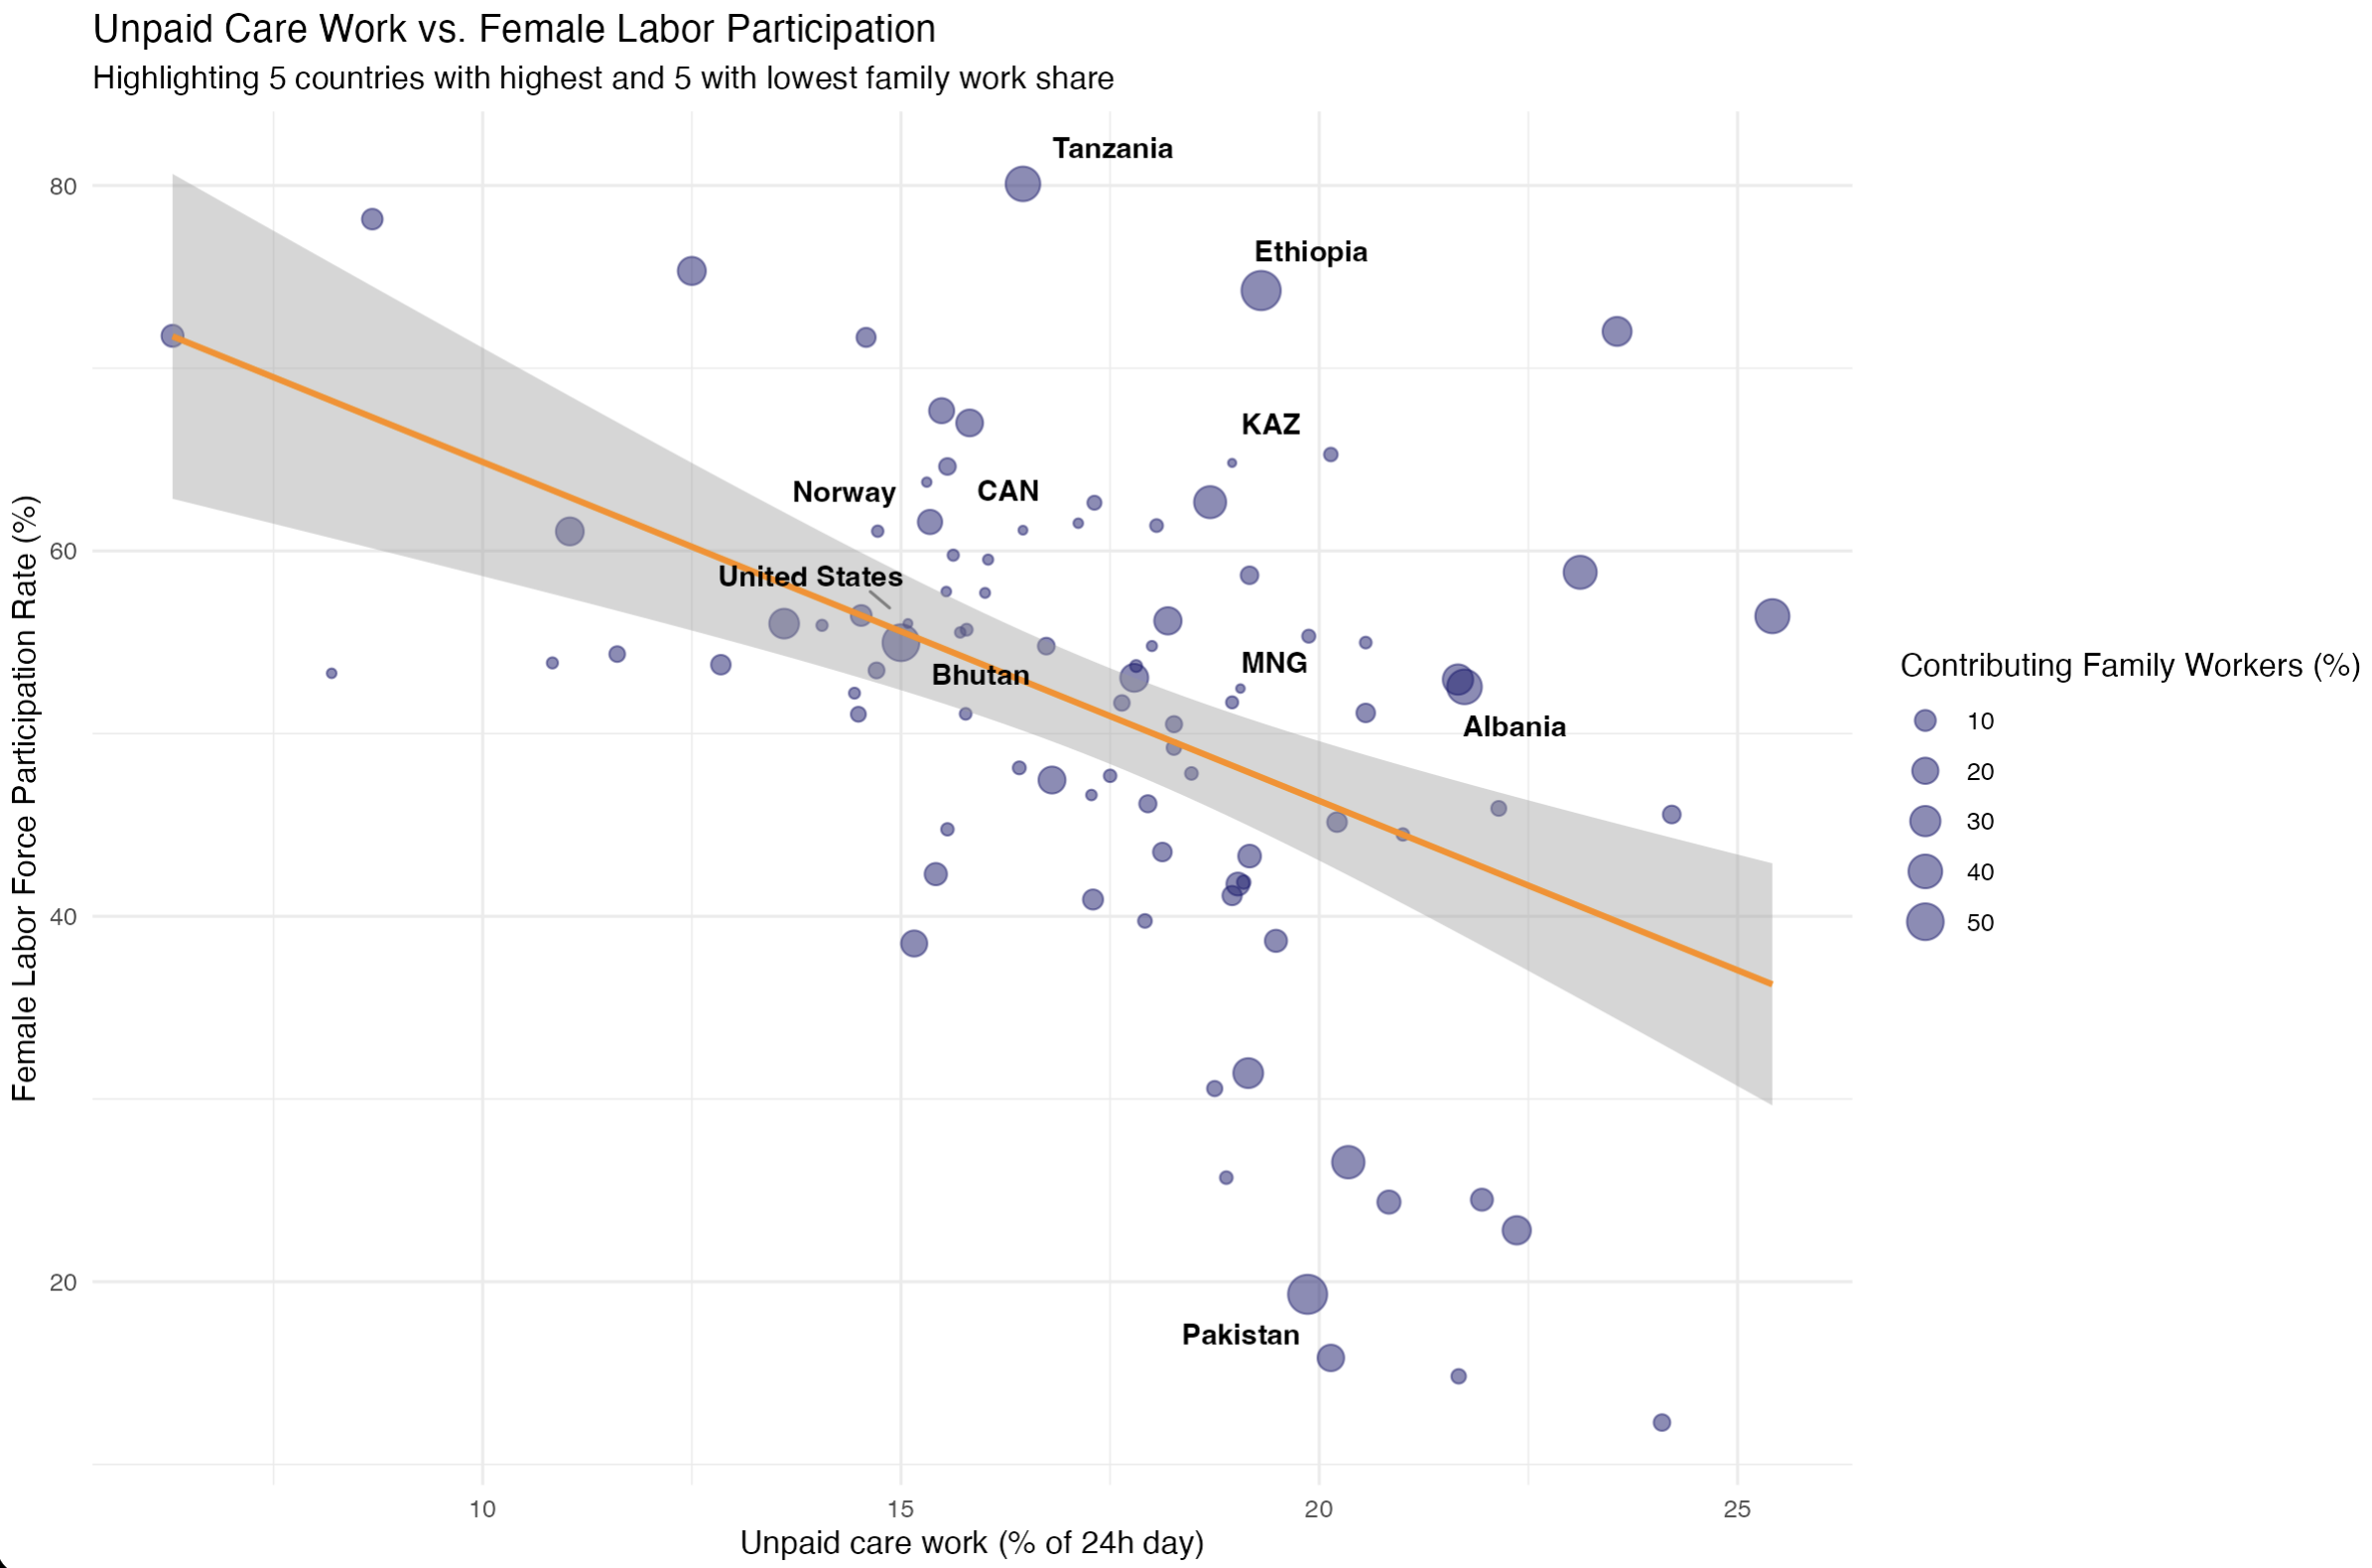
\includegraphics[keepaspectratio]{Final_Rplot.png}}

In contrast, the ``Low 5''---led by Norway (NWY) and its European
peers---reside in the upper-left quadrant. Here, we see the result of a
formalized social contract. The care burden is low (under 15\%), and
participation is high. Crucially, the bubble size is nearly
non-existent. In Norway, when a woman works, she is almost certainly an
employee with a contract, a bank account, and a social security number.
This transition from ``Family Worker'' to ``Employee'' is the pivotal
shift required for the financial inclusion of women globally.

\subsection{5. Conclusion: Efficiency, Power, and the ``Threat
Point''.}\label{conclusion-efficiency-power-and-the-threat-point.}

This project demonstrates that female labor participation is not an
isolated economic choice; it is the ``output'' of a domestic ``input''
of time. By building a transparent R-based pipeline, we have visualized
the ``Care Tax'' that suppresses women's economic potential.

5.1 The ``Society of Care'' as an Economic Efficiency Problem

One of the most significant conclusions of this analysis is that the
``Society of Care'' is not just a matter of social justice; it is a
matter of intra-household economic efficiency. As we have seen in our
results, the concentration of care in the ``Top 5'' countries suggests
that households are misallocating their most productive resources.

5.2 The Role of the ``Threat Point''

Following the theoretical framework of Jayachandran and Voena (2026), we
can conclude that while the care burden remains high, the ``threat
point'' (or reservation position) of women in the household remains
structurally weakened. This explains a critical phenomenon in our data:
even when the broader economy grows, the situation for women in
high-care burden countries does not automatically improve. Their
bargaining position is stagnant because they lack the ``time surplus''
necessary to accumulate independent assets. Without assets or formal
income, their ability to negotiate a better distribution of domestic
labour within the household is severely limited, creating a
self-perpetuating cycle of exclusion.

5.3 The Income Trap in the ``Top 5''

The massive bubbles observed in countries like Pakistan or Ethiopia
reveal a ``Trap of Income.'' In these contexts, control over resources
is what dictates power. Even when these women are recorded as
``working,'' their income---often informal or tied to family
enterprises---is frequently ``liquefied'' into immediate family
consumption. Unlike the formalized labor seen in Switzerland (Low 5),
this informal work does not generate individual financial autonomy.
Therefore, the ``Contributing Family Worker'' status is a statistical
veil that hides a lack of real economic agency.

In final reflection, the path to gender financial health must lead
through the redistribution of the care burden. Providing financial apps
or bank accounts is a superficial fix if the underlying ``Time Tax''
remains. We must move toward a policy horizon where time is treated as a
collective resource, ensuring that the ``Double Burden'' no longer
serves as the invisible ceiling for female economic empowerment.

\subsection{6. Critical Reflection and
Limitations}\label{critical-reflection-and-limitations}

No computational analysis is complete without a critical
self-assessment.

\begin{enumerate}
\def\labelenumi{\arabic{enumi}.}
\item
  The Statistical Silence: As observed during development, the World
  Bank API often returns NA for the ``Unpaid Care'' indicator in many
  regions. This ``data silence'' is a form of policy neglect.
\item
  Cultural Definitions of Care: The X-axis relies on self-reported data.
  In many households, caring for an elderly parent is seen as a
  ``natural'' family obligation rather than ``work,'' leading to a
  systematic underreporting of care hours.
\item
  The Limits of Linearity: While the orange trend line provides a useful
  average, social reality is often non-linear. Tipping points in
  infrastructure (like universal childcare) can cause non-linear
  explosions in labour participation.
\end{enumerate}

\subsection{Bibliography}\label{bibliography}

\begin{itemize}
\item
  BFA Global. (2026). Financial Health with a Gender Perspective:
  Resilience and Autonomy in Latin America. {[}Online Report{]}.
\item
  Jayachandran, S., \& Voena, A. (2026). Women's Power in the Household.
  NBER Working Paper Series, No.~34605.
\item
  World Bank. (2024). World Development Indicators: Unpaid Care Work
  (SG.TIM.UWRK.FE).
\item
  World Bank. (2024). World Development Indicators: Female Labor
  Participation (SL.TLF.CACT.FE.ZS).
\item
  World Bank. (2024). World Development Indicators: Contributing Family
  Workers (SL.FAM.WORK.FE.ZS).
\item
  R Core Team. (2023). R: A Language and Environment for Statistical
  Computing.
\item
  Slowikowski, K. (2023). ggrepel: Smart Labels for ggplot2. R package
  version 0.9.3.
\end{itemize}

\subsection{LLM Disclosure and Technical Assistance Note A Note on My
Use of AI in this
Project}\label{llm-disclosure-and-technical-assistance-note-a-note-on-my-use-of-ai-in-this-project}

As part of my commitment to academic transparency in the LUMACSS
program, I want to disclose that I teamed up with a Large Language Model
(LLM) to fine-tune the technical side of this research. While the core
ideas and analysis are mine, the AI acted as a ``digital lab assistant''
in the following ways:

\begin{itemize}
\item
  Audit and Cleanup of My R Scripts: I used the LLM to double-check my
  code logic, specifically to ensure that the WDI API calls were
  fetching data correctly and that my Most Recent Value (MRV) filtering
  was working as intended.
\item
  Documentation for Reproducibility: To make my work as accessible as
  possible for anyone trying to replicate it, I collaborated with the AI
  to write clear, detailed comments in English throughout my .R files.
\item
  Repository Organization: I followed AI-guided workflows to clean up my
  GitHub structure. This helped me programmatically create folders (like
  /scripts and /data\_preprocessed) and move files around without
  breaking the relative paths needed for the code to run.
\end{itemize}

Personal Responsibility and Intellectual Ownership It is important to
emphasize that I am the sole author of the conceptual framework and the
sociological interpretation of the results. The integration of sources
like Jayachandran \& Voena (2026) and the BFA Global report, as well as
the critical reflections on intra-household power dynamics and the
``Care Tax,'' are products of my own analysis. I used the AI to help me
build a better ``engine'' for the project, but the direction, the
``driver,'' and the final conclusions are entirely my own.

Technical Cheat Sheet:

Managing the GitHub Structure For my own future reference (or for anyone
replicating this work), here is how I managed the project environment
using the RStudio Console:

Creating Folders: I used if (!dir.exists(``name'')) dir.create(``name'')
to keep the workspace organized.

Moving Files: To keep the root directory clean, I moved scripts and
reports using file.rename(``old\_path/file.R'', ``scripts/file.R'').

Housekeeping: I removed temporary or redundant files with file.remove()
to ensure only the final, necessary data is hosted on GitHub.

Path Management: I used getwd() to verify my working directory, ensuring
that scripts inside the /scripts folder can correctly ``reach out'' to
data in /data\_preprocessed using the ../ notation.




\end{document}
